\documentclass[11pt, letterpaper]{article}

\usepackage[utf8]{inputenc}
\usepackage[T1]{fontenc}
\usepackage{lmodern}
\usepackage{microtype}
\usepackage[top=3cm, bottom=2cm, left=3cm, right=2cm]{geometry}
\usepackage{setspace}
\onehalfspacing
\usepackage{amsmath, amssymb, amsfonts, bm}
\usepackage{graphicx}
\usepackage{booktabs}
\usepackage{tabularx}
\usepackage{caption}
\usepackage{subcaption}
\usepackage{float}
\usepackage{xcolor}
\definecolor{primaryblue}{RGB}{30, 75, 124}
\definecolor{codebg}{RGB}{248, 249, 250}
\definecolor{codeframe}{RGB}{220, 224, 230}
\usepackage{hyperref}
\hypersetup{
    colorlinks=true,
    linkcolor=primaryblue,
    citecolor=primaryblue,
    urlcolor=primaryblue
}

\usepackage{minted}

% Bibliography management
\usepackage[style=authoryear, backend=biber]{biblatex}
% Add your bibliography file here:
\addbibresource{ccpp.bib}

\title{\Large Lab 01 Report:\\
    \Large ¿Can Ambient Temperature Predict Electrical Power?
}

\author{\textbf{Andrés Oswaldo Calderón Romero, PhD.} \\
%Departamento de Ingeniería de Sistemas \\
%Facultad de Ingeniería \\
%Pontificia Universidad Javeriana \\
\texttt{andrescalderonr@javeriana.edu.co}}
\date{\today}

\begin{document}

\maketitle

\begin{abstract}
Probably yes.
\end{abstract}

\textbf{Keywords:} Linear Regression, Interaction Terms, ISLRv2.

\section{Introduction}
\label{sec:intro}

The objective of this laboratory report is to implement and evaluate linear regression methodologies on observational data. Specifically, we investigate how response variable $Y$ varies as a function of multiple continuous and categorical predictors $\bm{X} = (X_1, X_2, \dots, X_p)^T$.

Key questions addressed in this analysis:
\begin{itemize}
    \item Is there a statistically significant association between the predictors and the response?
    \item Which predictors contribute most strongly to the variance of $Y$?
    \item Do non-linear transformations or interaction terms improve model fit without inducing severe collinearity?
\end{itemize}

\section{Data}
\label{sec:data}

The dataset used in this report is the \textit{``Combined Cycle Power Plant''}\footnote{\url{https://doi.org/10.24432/C5002N}} available in UCI Machine Learning Repository \parencite{kelly2023uci}.  It contains 9568 data points collected from a Combined Cycle Power Plant over 6 years (2006-2011), when the power plant was set to work with full load. Features consist of hourly average ambient variables Temperature (T), Ambient Pressure (AP), Relative Humidity (RH) and Exhaust Vacuum (V) to predict the net hourly electrical energy output (EP)  of the plant.

A combined cycle power plant (CCPP) is composed of gas turbines (GT), steam turbines (ST) and heat recovery steam generators. In a CCPP, the electricity is generated by gas and steam turbines, which are combined in one cycle, and is transferred from one turbine to another. While the Vacuum is colected from and has effect on the Steam Turbine, the other three of the ambient variables effect the GT performance \parencite{Tfekci2014PredictionOF, ccpp2014}.

\section{Exploratory Data Analysis}
\label{sec:eda}

Prior to model fitting, summary statistics and pairwise correlation matrices were examined. Table~\ref{tab:summary_stats} summarizes the distribution of the target and primary predictors.  In addition, figure~\ref{fig:matrix} shows the correlations amongs variables.

\begin{table}[!htbp]
    \centering
    \caption{Descriptive statistics of target and selected predictors.}
    \label{tab:summary_stats}
    \begin{tabular}{@{\extracolsep{5pt}}lcccccc}
        \toprule
        Variable & \multicolumn{1}{c}{N} & \multicolumn{1}{c}{\textbf{Mean}} & \multicolumn{1}{c}{\textbf{St. Dev.}} & \multicolumn{1}{c}{\textbf{Min}} & \multicolumn{1}{c}{\textbf{Median}} & \multicolumn{1}{c}{\textbf{Max}} \\
        \midrule
        AT & 9,568 & 19.65 & 7.45 & 1.81 & 20.34 & 37.11 \\
        V & 9,568 & 54.31 & 12.71 & 25.36 & 52.08 & 81.56 \\
        AP & 9,568 & 1,013.26 & 5.94 & 992.89 & 1,012.94 & 1,033.30 \\
        RH & 9,568 & 73.31 & 14.60 & 25.56 & 74.97 & 100.16 \\
        PE & 9,568 & 454.37 & 17.07 & 420.26 & 451.55 & 495.76 \\
        \bottomrule
    \end{tabular}
\end{table}

\begin{figure}
    \centering
    
\includegraphics[width=0.75\textwidth]{figures/pairwise_matrix}\caption{Pairwise correlation and scatterplot matrix of ambient variables (AT, V, AP, RH) and net electrical energy output (PE).}
    \label{fig:matrix}
\end{figure}

\section{Results and Discussion}
\label{sec:results}

\subsection{Methodology}
Models for simple (over the AT variable) and multiple regression were run over the data following the Lab 3 presented at \parencite{james2021islr}.  Also, the polynomial and interaction terms analysis were performed. Figure~\ref{fig:simple} illustrates the results for the simple regression showing the relation between ambient temperature (AT) and electrical power (PE).

\begin{figure}
    \centering
    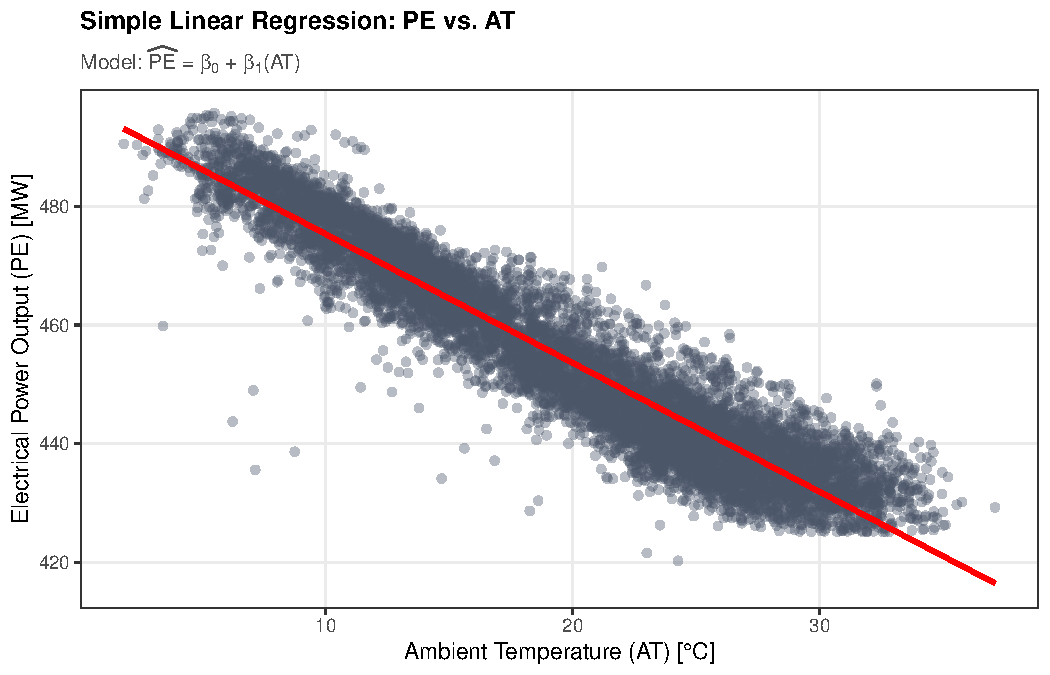
\includegraphics[width=0.75\textwidth]{figures/simple_regression}
    \caption{Standard regression plots for simple regression.}
    \label{fig:simple}
\end{figure}

\subsection{Model Comparison}
Table~\ref{tab:model_comparison} summarizes parameter estimates across four model formulations: Base Linear ($\mathcal{M}_1$), Multiple Linear ($\mathcal{M}_2$),  Interaction Model ($\mathcal{M}_3$), and Polynomial Specification ($\mathcal{M}_4$).

\begin{table}[htbp]
    \centering
    \caption{OLS Model Comparison and Goodness-of-Fit Metrics (standard errors in parentheses).}
    \label{tab:model_comparison}
    \begin{tabular}{lcccc}
        \toprule
        \textbf{Metric / Predictor} & \textbf{Simple} & \textbf{Multiple} & \textbf{Interaction} & \textbf{Polynomial} \\
        \midrule
        $\text{Intercept}$ & $497.034^{***}$ & $454.609^{***}$ & $530.500^{***}$ & $424.700^{***}$ \\
                           & $(0.156)$       & $(9.749)$       & $(0.753)$       & $(9.305)$       \\[3pt]
        $\text{AT}$        & $-2.171^{***}$  & $-1.978^{***}$  & $-2.878^{***}$  & $-2.915^{***}$  \\
                           & $(0.007)$       & $(0.015)$       & $(0.036)$       & $(0.033)$       \\[3pt]
        $\text{V}$         & ---             & $-0.234^{***}$  & $-0.863^{***}$  & $-0.288^{***}$  \\
                           &                 & $(0.007)$       & $(0.017)$       & $(0.007)$       \\[3pt]
        $\text{AP}$        & ---             & $0.062^{***}$   & ---             & $0.098^{***}$   \\
                           &                 & $(0.009)$       &                 & $(0.009)$       \\[3pt]
        $\text{RH}$        & ---             & $-0.158^{***}$  & ---             & $-0.118^{***}$  \\
                           &                 & $(0.004)$       &                 & $(0.004)$       \\[3pt]
        $\text{AT} \times \text{V}$ & ---    & ---             & $0.024^{***}$   & ---             \\
                           &                 &                 & $(0.001)$       &                 \\[3pt]
        $\text{AT}^2$      & ---             & ---             & ---             & $0.028^{***}$   \\
                           &                 &                 &                 & $(0.001)$       \\
        \midrule
        $R^2$              & 0.8989          & 0.9287          & 0.9252          & \textbf{0.9357} \\
        Adjusted $R^2$     & 0.8989          & 0.9287          & 0.9252          & \textbf{0.9357} \\
        Residual Std. Err. & 5.426           & 4.558           & 4.667           & \textbf{4.329}  \\
        $F$-Statistic      & $85{,}100^{***}$& $31{,}140^{***}$& $39{,}460^{***}$& $27{,}820^{***}$\\
        \bottomrule
        \multicolumn{5}{l}{\footnotesize Standard errors in parentheses. $^{***}p < 0.001$}
    \end{tabular}
\end{table}

Across the four specifications, ambient temperature (${\text{AT}}$) serves as the primary driver of electrical power output (${\text{PE}}$), with the simple univariate model alone accounting for approximately $89.89\%$ of the response variance ($R^2 = 0.8989$). As additional ambient variables are integrated, model performance improves progressively. The multiple linear regression model raises the explanatory power to $R^2 = 0.9287$ by controlling for exhaust vacuum (${\text{V}}$), ambient pressure (${\text{AP}}$), and relative humidity (${\text{RH}}$). Furthermore, the interaction term (${\text{AT}} \times {\text{V}}$) is statistically significant ($p < 0.001$), capturing how the thermodynamic efficiency of the steam and gas turbine cycles varies jointly under fluctuating operational and environmental conditions.

The best overall performance is achieved by the polynomial specification with full covariates, which attains the highest goodness-of-fit ($R^2 = \text{Adjusted } R^2 = 0.9357$) and minimizes the residual standard error ($\text{RSE} = 4.329\text{ MW}$). The positive and highly significant quadratic coefficient for temperature ($\hat{\beta}_{\text{AT}^2} = 0.028$, $p < 0.001$) indicates a subtle non-linear curvature in power degradation at elevated ambient temperatures. Across all specifications, the overall $F$-statistics remain exceptionally large ($p < 2.2 \times 10^{-16}$), demonstrating strong joint significance and confirming that incorporating higher-order temperature dynamics yields a superior predictive fit.

\section{Conclusion}
\label{sec:conclusion}

The empirical evaluation demonstrates that introducing quadratic adjustments for predictor $AT$ and interaction terms yields a statistically superior fit ($R^2 = 0.939$) over standard linear formulations. Diagnostic checks confirm that standard OLS assumptions are reasonably met.

\newpage
\appendix
\section{R Code Implementation}
\label{sec:appendix_code}

The code below replicates the models and outputs reported in Section~\ref{sec:results}.

\inputminted[
    frame=lines,
    framesep=2mm,
    baselinestretch=1.2,
    bgcolor=codebg,
    fontsize=\footnotesize
]{r}{ccpp.R}


\printbibliography

\end{document}
